\documentclass[10pt]{article}

\usepackage[]{hyperref}
\usepackage{amsmath} 
\usepackage{amsfonts} 
\usepackage{anysize} 
\usepackage{graphicx}
\usepackage{hyperref}
\usepackage{cite}
\usepackage{caption}
\usepackage{url}
\usepackage{t1enc}  
\usepackage{wrapfig}
\usepackage{mathtools,amssymb}
%\usepackage{palatino}

\renewcommand{\topfraction}{.95}  % max fraction of floats at top
\renewcommand{\bottomfraction}{.95}       % max fraction of floats at bottom
    \setcounter{topnumber}{4}
    \setcounter{bottomnumber}{4}
    \setcounter{totalnumber}{4}     % 2 may work better
    \setcounter{dbltopnumber}{2}    % for 2-column pages
    \renewcommand{\dbltopfraction}{1}   % fit big float above 2-col. text
    \renewcommand{\textfraction}{0.05}  % allow minimal text w. figs
    %   Parameters for FLOAT pages (not text pages):
    \renewcommand{\floatpagefraction}{0.95}     % require fuller float pages
        % N.B.: floatpagefraction MUST be less than topfraction !!
    \renewcommand{\dblfloatpagefraction}{0.95}  % require fuller float pages

\newenvironment{myitemize}{\begin{itemize} \setlength{\topsep}{0pt} \setlength{\itemsep}{0pt} \setlength{\parskip}{0pt} \setlength{\parsep}{0pt}}{  \end{itemize} }
\setlength{\itemsep}{0pt}
\newenvironment{myenumerate}{\begin{enumerate} \setlength{\topsep}{0pt} \setlength{\itemsep}{0pt} \setlength{\parskip}{0pt} \setlength{\parsep}{0pt} }{  \end{enumerate} }

\begin{document}

\title{Summary for the RecSys 2017 Online Ranking Tutorial}
\date{\vspace{-0.1cm}}
\maketitle

\section{Rating and ranking prediction}

A common definition for the recommendation task is the \emph{rating prediction} problem.
For a given user $u$ and a given item $i$ the system should return a predicted relevance $\hat{r}_{ui}$.
The actual preference of the user on the item is $r_{ui}$.
While the rating prediction task is highly popular, the top-$K$ \emph{ranking prediction} problem is closer to the actual industrial use-cases.
In this setting, for a given user $u$ the recommender should retrieve an ordered set of relevant items $\lbrace {i_1, i_2, ..., i_K}\rbrace$, where the number of returned items is $K$.

\section{Classes of recommendation algorithms}

\begin{myitemize}
\item \textbf{Content-based} recommenders use user profiles and item content for recommendation, for example the description of a product, or information on the user in a social network.

\item \textbf{Collaborative filtering} (CF) methods use historical data that contain the past interactions of the users and the items logged by the service provider.
One type of CF algorithms are matrix factorization (MF) models that map the users and the items to a lower $k$ dimensional space.

\item \textbf{Context-aware} recommenders not only investigate user-item interactions, but also their conditions.
Contextual information mainly describes the user and in general user-item interactions, e.g. the updated location information of the user.
\end{myitemize}
\section{Explicit and implicit recommendation}

Recommendation scenarios can differ based on the type of data available for training.
Collaborative filtering methods learn by investigating the interactions between the users and the items.
When the data contains ratings e.g. on a scale between 1-5, the problem is an explicit recommendation task.
In case of implicit feedback, there is no exact information about the user preferences, e.g.\ only the click history of the user is known. 

\section{Matrix factorization}
\label{sec:mf}

Matrix factorization models~\cite{koren2009matrix} are collaborative filtering methods that use the past interactions between the users and the items.
Those can be mapped to a user-item matrix, the utility matrix $R$ (see Fig.~\ref{fig:utility-matrix}).
Each row of $R$ corresponds to a given user, and each column corresponds to a given item.
In case of explicit feedback, $r_{ui}$ is the value of the rating given by user $u$ for item $i$.
For implicit feedback, $r_{ui}$ is equal to 1 if user $u$ previously interacted (clicked, viewed, \ldots) item $i$.

Note that $R$ is a sparse matrix, and most of its elements are unknown.
The task of the recommender algorithm is to predict correctly the unknown part of the matrix.
To achieve this, MF models decompose $R$ into two dense matrices $P$ and $Q$.
For a given user $u$, the corresponding row in $P$ is the user vector $p_u$.
For item $i$, the corresponding column of $Q$ is the item vector $q_i$.
The predicted relevance of item $i$ for user $u$ is then
\begin{equation}
	\hat{r}_{ui} = p_u q_i^T.
\end{equation}

\begin{figure}
\centering
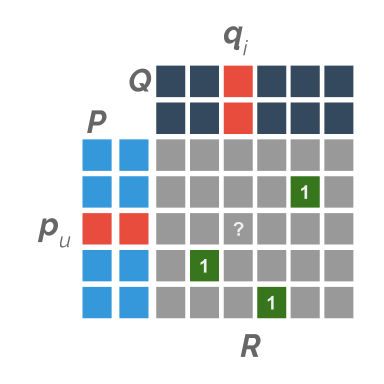
\includegraphics[width=5cm]{./figs/mf.pdf}
\caption{The utility matrix $R$ and the matrix factorization model built from matrix $P$ and $Q$.}
\label{fig:utility-matrix}
\end{figure}

\subsection{Optimization by stochastic gradient descent}

We introduce an algorithm that learns the model parameter matrices $P$ and $Q$~\cite{koren2009matrix}.
For the utility matrix $R$ that contains a set of ratings T, we intend to minimize the L2 norm of the difference between predicted relevances and the actual ratings,
\begin{equation}
F = \displaystyle\sum_{r_{ui} \in \text{T}} \left ( r_{ui} - \hat{r}_{ui} \right ) ^ 2,
\label{eq:mse}
\end{equation} 
i.e.\ the objective function that we optimize for is the mean squared error (MSE) on the training set.
For searching the minimum, we use stochastic gradient descent (SGD) that iterates several times on the known user-item ratings in the training set.
For a given $(u,i)$, the steps of the algorithm are the following.
\begin{myitemize}
\item We compute the gradient of the objective function $F$ with respect to the model parameters,
\begin{gather}
	\frac{\partial F}{\partial p_u} =   - 2 (r_{ui} - \hat{r}_{ui}) q_i, \hspace{1cm}
	\frac{\partial F}{\partial q_i} =   - 2 (r_{ui} - \hat{r}_{ui}) p_u.
\end{gather}
\item Then we take a step and update the model parameters towards the direction opposite to the gradient. The step is proportional to the learning rate $\eta$,
\begin{gather}
	p_u \leftarrow  \eta (r_{ui} - \hat{r}_{ui}) q_i, \hspace{1cm}
	q_i \leftarrow  \eta (r_{ui} - \hat{r}_{ui}) p_u.
\end{gather}
\end{myitemize}

\subsection{Variants of matrix factorization}
\label{sec:mf-variants}

Learning algorithms can vary by the their model, objective function, and their optimization algorithm.
Previously we learned a matrix factorization model by applying SGD to minimize the MSE in equation \eqref{eq:mse}.
Next we list some popular modifications of MF models.

\textbf{L2 regularization:}  A general way to avoid overfitting is to modify the objective function with a regularization term~\cite{koren2009matrix},
\begin{equation}
	\tilde{F} = F + F_{\text{reg}} = \displaystyle\sum_{r_{ui} \in \text{T}} \left ( r_{ui} - \hat{r}_{ui} \right ) ^ 2 + \lambda \left [ |p_u|^2 + |q_i|^2 \right ].
	\label{eq:obj-reg}
\end{equation}
The modified update rules are then
\begin{gather}
	p_u \leftarrow  \eta (r_{ui} - \hat{r}_{ui}) q_i - \eta \lambda p_u, \hspace{1cm}
	q_i \leftarrow  \eta (r_{ui} - \hat{r}_{ui}) p_u - \eta \lambda q_i.
\end{gather}

\textbf{Bias terms:}  
One can modify the model by introducing scalar terms that describe the biased behavior of the users and the items~\cite{koren2009matrix},
\begin{equation}
	\hat{r}_{ui} = b_u + b_i + p_u q_i^T,
\end{equation}
where $b_u$ is the user bias term and $b_i$ is the item bias term. Both parameters can be fit by SGD.

\textbf{Negative sampling:}  
In case of implicit feedback, the known part of the utility matrix only contains constant 1 elements.
To fit a model, one has to assume that at least part of the unknown part is 0, i.e.\ for some unknown elements, the user has not interacted with the items because she did not prefer them.
In case of SGD, we sample $C$ times more samples than positive ones from the unknown elements uniformly and learn $r_{ui} = 0$ for those ``negative samples''.
%When applying SGD for learning, this assumption is computationally efficient and the algorithm iterates on each record once.
%If we generate $C$ times more negative samples than positive ones, then the computational time is only multiplied by the constant factor $C$.

\textbf{Confidence values:}  
In an implicit ratings prediction task, one can introduce lower confidence values for the unknown negative events~\cite{hu2008collaborative}.
In contrast to negative sampling, we include all user-item pairs in the objective function, but  with different confidence $c_{ui}$ as
\begin{equation}
\tilde{F'} = \displaystyle\sum_{u,i} c_{ui} \left ( r_{ui} - \hat{r}_{ui} \right ) ^ 2 + \lambda \left [  \displaystyle\sum_u | p_u | ^ 2 + \displaystyle\sum_i |q_i| ^ 2\right],
\label{eq:obj-reg-all}
\end{equation}
where we set $c_{ui} = c > 1$ for user-item pairs where $r_{ui}>0$ (e.g.\ $c:=40$), and  $c_{ui}: = 1 $ when $r_{ui} = 0$.

%%\textbf{Pairwise ranking:}  
%%By using the mean squared error for objective function, one cannot optimize directly for top recommendation.
%%While there exist several objectives for ranking prediction, generally they are non-differentiable.
%%Rendle et al.~\cite{rendle2009bpr} proposed the Bayesian Personalized Ranking (BPR) algorithm. 
%%While BPR operates with the familiar MF model and learns the model parameters with SGD, it introduces a new objective function
%%\begin{equation}
	%%F_{BPR} = \displaystyle\sum_{\lbrace (u,i,j) |  i \in S_u  \wedge j \notin S_u \rbrace} \ln \sigma (\hat{r}_{ui}-\hat{r}_{uj}),
%%\end{equation}
%%where $S_u$ is the set of ratings given by user $u$, and $\sigma$ is the sigmoid function.
%%Note that this objective is defined over pair of ratings.

%%\textbf{Asymmetric matrix factorization:}  
%%In case of asymmetric matrix factorization, we modify the original factorization model by introducing another dense matrix $A$ instead of $P$~\cite{patarekamf}.
%%The $j$th row of $A$ corresponds to item $j$.  
%%For a given ($u$,$i$) pair, the prediction is then
%%\begin{equation}
	%%\hat{r}_{ui} = \left [ \frac{1}{\sqrt{|S_u|}} \displaystyle\sum_{j \in S_u} a_j \right ]  q_i,
%%\end{equation}
%%where $S_u$ is the set of items viewed by user $u$.
%%Note that instead of a single vector, we model the user by the sum of vectors from $A$ corresponding to items previously rated by her.
%%For a new incoming user with only a few interactions this is beneficial: her latent vector is then the sum of item vectors that may already incorporate several updates from the interactions of other users.

\textbf{ALS:}  
The alternating least squares method~\cite{pilaszy2010fast,koren2009matrix} (ALS) is another preferred algorithm besides SGD. 
The concept of ALS is that for a fixed $Q$ it computes the best $P$ i.e. $P$ that minimizes the objective function.
Then for a fixed $P$ it calculates the best $Q$.
We continue this iteration until we get satisfactory objective values.
More specifically, we use the objective function in~\eqref{eq:obj-reg}.
When we fix $Q$, this defines a separate optimization problem for each user $u$.
The objective for a particular user $u$ is then
\begin{equation}
	\tilde{F_u} = \displaystyle\sum_{i:(u,i) \in \text{T}} 2 \left (r_{ui} - p_u q_i^T \right ) ^ 2 + \lambda |p_u|^2.
	\label{eq:als-obj}
\end{equation}
Next we introduce some notations for user $u$,
\begin{myitemize}
	\item $S_u = \{r_{ui_1}, r_{ui_2}, ..., r_{ui_s}\}$ is the set of the items rated by $u$, $s:=|S_u|$,
	\item $b_u:=\left [ r_{ui_1}, r_{ui_2}, ..., r_{ui_s} \right ]$ is the rating vector of $u$,
	\item $Q_u:=\left [ q_{i_1}^T, q_{i_2}^T, ..., q_{i_s}^T \right ]$ is the matrix constructed from the latent vectors of the items rated by $u$.
\end{myitemize}
Equation \eqref{eq:als-obj} can be rewritten as
\begin{equation}
	\tilde{F_u} = | b_u - p_u Q_u | ^ 2 + \lambda |p_u|^2.
\end{equation}
The optimal $p_u$ can be found by solving $\frac{\partial\tilde{F_u}}{\partial p_u}:=0$,
\begin{equation}
	\frac{\partial\tilde{F}}{\partial p_u} = 2 Q_u^T(p_u Q_u - b_u )+ 2 \lambda p_u = 0,
\end{equation}
therefore the final solution for $p_u$ is
\begin{equation}
	p_u = (Q_u Q_u^T + \lambda I_s)^{-1} Q_u^T b_u,
\end{equation}
where $I_s$ is the $s$-dimensional identity matrix.
Similarly, the update step for each item $i$ is
\begin{equation}
	q_i = (P_i P_i^T + \lambda I_s)^{-1} P_i^T b_i,
\end{equation}
where the definitions of $P_i$ and $b_i$ are similar to the definitions of $Q_u$ and $b_u$.  

\textbf{iALS:}  
Koren et al.~\cite{hu2008collaborative} proposed a variant of the original ALS algorithm for an implicit setting.
We use the objective function with confidence values and regularization~\eqref{eq:obj-reg-all} that contains \emph{all} elements in $R$.
We apply a similar alternating algorithm for computing the user and the item vectors as in case of ALS.
Equation~\eqref{eq:obj-reg-all} can be rewritten as
\begin{equation}
	\tilde{F'} = \displaystyle\sum_u \left | \sqrt{C^u} r_u - \sqrt{C^u} Q p_u \right | ^ 2 + \lambda \left [  \displaystyle\sum_u | p_u | ^ 2 + \displaystyle\sum_i |q_i| ^ 2\right],
\end{equation}
where
\begin{myitemize}
\item $r_u:= \left [ r_{u1}, r_{u2}, ..., r_{uM} \right ]$ is a vector that contains the preferences of user $u$ and $M$ is the total number of items,
\item $C_u$ is a $N \times N$ diagonal matrix containing the confidence values of $u$ in the diagonal.
\end{myitemize}
The optimal $p_u$ can be set by solving $\frac{\partial\tilde{F'}}{\partial p_u}:=0$,
\begin{equation}
	\frac{\partial \tilde{F'} }{\partial p_u} =  2 \left [ Q^T C^u Q p_u  - Q^T C^u r_u \right ]  + 2 \lambda p_u.
\end{equation}
As for a fixed $Q$ for the optimal $p_u$  $\frac{\partial \tilde{F'} }{\partial p_u} = 0$,
\begin{equation}
	p_u =  \left [ Q^T C^u Q + \lambda I \right ] ^ {-1} Q^T C^u r_u.
	\label{eq:als_u}
\end{equation}
Similarly for a fixed $P$, the optimal $q_i$ is
\begin{equation}
	q_i =  \left [ P^T C^i P + \lambda I \right ] ^ {-1} P^T C^i r_i,
	\label{eq:als_i}
\end{equation}
where  vector $r_i$ contains the preferences for item $i$, and $C_i$ is a diagonal matrix containing the confidence values for $i$.

To sum up, we compute the user vectors and the item vectors in an alternating way based on~\eqref{eq:als_u} and~\eqref{eq:als_i}.
Note that a significant speedup can be achieved by rewriting these expressions to 
\begin{gather}
		p_u =  \left [ Q^T Q + Q^T [C^u  - I ] Q + \lambda I \right ] ^ {-1} Q^T C^u r_u\text{ and }
		q_i =  \left [ P^T P + P^T [C^i - I] P + \lambda I \right ] ^ {-1} P^T C^i r_i.
\end{gather}

\section{Evaluation metrics}

A usual setting for evaluation is to divide the available data set into a training and an evaluation set.
We learn the parameters of our model on the training set $T$, and evaluate its performance on a separated evaluation set $E$.
%Here we list standard evaluation metrics of recommender systems in this setting.
%We assume that a separated evaluation set $E$ is given that contains ratings $r_{ui}$.
%We consider explicit rating and implicit ranking prediction problems.

\subsection{Explicit rating prediction}

The metric used in the Netflix Prize competition is a natural choice: the mean squared error simply computes the squared difference of the predicted and actual ratings,
\begin{equation}
	MSE = \displaystyle\sum_{(u,i) \in \text{E}}  ( \hat{r}_{ui} - r_{ui} ) ^ 2,
\end{equation}
where the error is computed on the evaluation set of ratings $E$.

\subsection{Implicit ranking prediction}

In this setting the recommender should return an ordered top-$K$ list of items $L_u$ for a given user $u$.
We compare the top list $L_u$ in question against the items consumed by the user in the evaluation set $E_u$.
Precision and recall are standard information retrieval metrics that can be applied for ranking evaluation.
For a given user $u$,
\begin{equation}
	\text{Precision@K}_u = \frac{|E_u \cap L_u|}{K}, \hspace{3cm}  \text{Recall@K}_u = \frac{|E_u \cap L_u|}{|E_u|}.
\end{equation}

While precision@K and recall@K are widely used, they do not consider the rank of the relevant items.
In contrast, mean average precision@K (MAE@K) depends on the ranking of the items in the list, 
\begin{equation}
	\text{MAE@K} = \frac{1}{K} \displaystyle\sum_{k=1}^K  \text{precision@k}.
\end{equation}
A more standard ranking based metric is discounted cumulative gain@K (DCG@K),
\begin{equation}
	\text{DCG@K} = \displaystyle\sum_{k=1}^K \frac{\text{rel}(i_k)}{\log_2(1 + k)}
	\label{eq:dcg}
\end{equation}
where $\text{rel}(i_k)$ notes the relevance of the i-th item in the list.
For the implicit task, the relevance is 1 if the user considered the item in the evaluation set, otherwise it is 0.
%If we define iDCG@K, the ideal maximum possible value of DCG@K for the given user, then we may obtain nDCG@K, the normalized version of DCG@K as
%\begin{equation}
%\text{nDCG@K} = \frac{\text{DCG@K}}{\text{iDCG@K}}.
%\label{eq:ndcg}
%\end{equation}

\section{The online ranking prediction problem}
\label{sec:ranking-prediction}

%In this section we address the implicit top-$k$ recommendation task~\cite{cremonesi2010performance}.%where the goal is not to rate some of the individual items but to provide the best candidates.
In a time sensitive or online recommender that potentially re-trains the model after each and every new item, we have to generate a new top-$k$ recommendation list for every single event in the evaluation period.
%The online top-$k$ task is hence different from the standard recommender evaluation settings, since there is always a single relevant item only in the ground truth.
In an online setting, as seen in Figure~\ref{fig:online},
\begin{myenumerate}
\item we query the recommender for a top-$k$ recommendation for the active user,
\item we evaluate the list in question against the single relevant item that the user interacted with,
\item we allow the recommender to train on the revealed user-item interaction.
\end{myenumerate}

\begin{figure}
\centering
\includegraphics[width=9cm]{./figs/online.pdf}
\caption{Temporal evaluation of the online ranking prediction problem.}
\label{fig:online}
\end{figure}

\section{Average DCG for online evaluation}

We show that DCG computed \emph{individually} for each event and averaged in time is an appropriate measure for real-time recommender evaluation.
If $i$ is the next consumed item by the user, the online DCG@K is defined as the following function of the rank of $i$ returned by the recommender system,
\begin{equation}
  \mbox{DCG@K}(i) = 
     \begin{cases}
        0 & \mbox{if rank}(i) > K; \\
        \frac{\displaystyle 1}{\displaystyle \log_2 (\mbox{rank}(i)+1)} & \mbox{otherwise}.
     \end{cases}
  \label{eq:online-dcg}
\end{equation}
The overall evaluation of a model is the average of the DCG@K values over all events of the evaluation period.
Furthermore, evaluating each event in the time series allows us to measure timely averages over the dataset, e.g. we may compute daily average DCG scores.

\section{Online matrix factorization}
\label{sec:online-mf}

As originally designed, stochastic gradient descent methods may iterate several times over the training set until convergence.
In an real-time recommendation task, however, the model needs to be re-trained after each new event and hence re-iterations over the earlier parts of the data may be computationally infeasible.
We may implement an online recommender algorithm by allowing a \emph{single} iteration over the training data only when we process the events in \emph{temporal} order.
%Online recommenders seem more restricted than those that may iterate over the data set several times and one could expect inferior quality by the online methods.
%Online methods however have the advantage of having much more emphasis on recent events.

Specifically for online matrix factorization we may set MSE as the objective function and we can apply online SGD for learning.
In an implicit setting we may use the following sampling technique:
\begin{myitemize}
\item When we update the model for the most recent positive record, we generate $C$ random negative samples for the given user.
\item After performing the update steps for the positive record, we process the negative samples with rating assigned to be 0.
\item We exclude items that appeared before the time of the positive interaction when generating negative samples.
\end{myitemize}

\section{Online combination}
\label{sec:online-combination}

We give an SGD based method to learn the online combination weight of recommender algorithms.
More specifically,
\begin{myitemize}
	\item we intend to linearly combine the output of $M$ models,
	\item each model $m$ should return a score $\hat{r}_{ui}^m$,
	\item the global combination weight of model $m$ is $\alpha_m$,
	\item for user $u$ the personalized combination weight is $\beta_m^u$,
	\item we learn the parameters $\alpha_m$ and $\beta_m^u$ by online SGD.
\end{myitemize}
We optimize for
\begin{equation}
F_{\text{C}}= \left ( r_{ui} - \displaystyle\sum_m (\alpha_m + \beta_m^u) \hat{r}^m_{ui}\right )^2.
\end{equation}
In this setting (1) we iterate over each record in the data set in temporal order, (2) we generate negative samples for each implicit record, (3) we learn the combination weights by online SGD. The corresponding derivatives are
\begin{gather}
\frac{\partial F}{\partial \alpha_m} = \frac{\partial F}{\partial \hat{r}_{ui}} \frac{\partial \hat{r}_{ui}}{\partial \alpha_m} = \frac{\partial F}{\partial \hat{r}_{ui}} \hat{r}_{ui}^m, \hspace{1cm}
  \frac{\partial F}{\partial \beta_m^u} = \frac{\partial F}{\partial \hat{r}_{ui}} \frac{\partial \hat{r}_{ui}}{\partial \beta_m^u} = \frac{\partial F}{\partial \hat{r}_{ui}} \hat{r}_{ui}^m.
\end{gather}

\begin{thebibliography}{10}

%\bibitem{netflix-prize}
%James Bennett and Stan Lanning.
%\newblock The netflix prize.
%\newblock In {\em KDD Cup and Workshop in conjunction with KDD 2007}, 2007.

%\bibitem{cremonesi2010performance}
%P.~Cremonesi, Y.~Koren, and R.~Turrin.
%\newblock Performance of recommender algorithms on top-n recommendation tasks.
%\newblock In {\em Proceedings of the fourth ACM conference on Recommender
%  systems}, pages 39--46. ACM, 2010.

%\bibitem{funk2006netflix}
%Simon Funk.
%\newblock Netflix update: Try this at home, 2006.

\bibitem{hu2008collaborative}
Yifan Hu, Yehuda Koren, and Chris Volinsky.
\newblock Collaborative filtering for implicit feedback datasets.
\newblock In {\em Data Mining, 2008. ICDM'08. Eighth IEEE International
  Conference on}, pages 263--272. IEEE, 2008.

%\bibitem{koenigstein2013towards}
%Noam Koenigstein and Yehuda Koren.
%\newblock Towards scalable and accurate item-oriented recommendations.
%\newblock In {\em Proceedings of the 7th ACM conference on Recommender
%  systems}, pages 419--422. ACM, 2013.

\bibitem{koren2009matrix}
Yehuda Koren, Robert Bell, and Chris Volinsky.
\newblock Matrix factorization techniques for recommender systems.
\newblock {\em Computer}, (8):30--37, 2009.

\bibitem{palovics2014exploiting}
R{\'o}bert P{\'a}lovics, Andr{\'a}s~A Bencz{\'u}r, Levente Kocsis, Tam{\'a}s
  Kiss, and Erzs{\'e}bet Frig{\'o}.
\newblock Exploiting temporal influence in online recommendation.
\newblock In {\em Proceedings of RecSys 2014}, pages 273--280. ACM, 2014.

%\bibitem{patarekamf}
%Arkadiusz Paterek.
%\newblock Improving regularized singular value decomposition for collaborative
%  filtering.
%\newblock In {\em Proc. KDD Cup Workshop at SIGKDD'07, 13th ACM Int. Conf. on
%  Knowledge Discovery and Data Mining}, pages 39--42, 2007.

\bibitem{pilaszy2010fast}
Istv{\'a}n Pil{\'a}szy, D{\'a}vid Zibriczky, and Domonkos Tikk.
\newblock Fast als-based matrix factorization for explicit and implicit
  feedback datasets.
\newblock In {\em Proceedings of the fourth ACM conference on Recommender
  systems}, pages 71--78. ACM, 2010.

%\bibitem{rendle2009bpr}
%Steffen Rendle, Christoph Freudenthaler, Zeno Gantner, and Lars Schmidt-Thieme.
%\newblock Bpr: Bayesian personalized ranking from implicit feedback.
%\newblock In {\em Proceedings of the twenty-fifth conference on uncertainty in
%  artificial intelligence}, pages 452--461. AUAI Press, 2009.

\end{thebibliography}


\end{document}
